\documentclass[conference]{IEEEtran}
\IEEEoverridecommandlockouts
% The preceding line is only needed to identify funding in the first footnote. If that is unneeded, please comment it out.
\usepackage{lscape}
\usepackage[table,xcdraw]{xcolor}
\usepackage{hyperref}
\hypersetup{colorlinks=true,allcolors=blue}
\usepackage{cite}
\usepackage{amsmath,amssymb,amsfonts}
\usepackage{algorithmic}
\usepackage{graphicx}
\graphicspath{{figures/}}
\usepackage{textcomp}
\usepackage{xcolor}
\def\BibTeX{{\rm B\kern-.05em{\sc i\kern-.025em b}\kern-.08em
    T\kern-.1667em\lower.7ex\hbox{E}\kern-.125emX}}
\begin{document}

\title{Understanding Learning Behaviours in\\
   Sorting Algorithm Game
}
%\thanks{Identify applicable funding agency here. If none, delete this.}
%}

\author{\IEEEauthorblockN{1\textsuperscript{st} Alfa Yohannis}
\IEEEauthorblockA{\textit{Department of Informatics} \\
\textit{KALBIS Institute}\\
Jakarta, Indonesia \\
alfa.yohannis@kalbis.ac.id}
\and
\IEEEauthorblockN{2\textsuperscript{nd} Kembang Goreng}
\IEEEauthorblockA{\textit{Department of Informatics} \\
  \textit{KALBIS Institute}\\
  Jakarta, Indonesia \\
  kembang.goreng@kalbis.ac.id}
\and
\IEEEauthorblockN{3\textsuperscript{rd} Pertanyaan Pernyataan}
\IEEEauthorblockA{\textit{Department of Informatics} \\
  \textit{KALBIS Institute}\\
  Jakarta, Indonesia \\
  pertanyaan.pernyataan@kalbis.ac.id}
}

\maketitle

\begin{abstract}
Based on our previous work, our gamification of sorting algorithm learning has been able to support learners to produce better learning outcomes if we compare them to the performance when they learn only in a traditional way – using textbooks. However, the finding does not reveal any specific explanation of how the result could happen. In this research, we make an effort to identify several learning behaviours and examine to what extent they can lead learners to successful learning outcomes. Therefore, we extract several variables as the representation of the learning behaviours and outcomes from the event logs. We calculate the correlations between the variables and identify that: allocating efforts on understanding the algorithms didactically, paying attention to the demo or illustration, spending more time playing, and exerting more attempts to complete the levels correlate significantly and positively with varying magnitudes to the completeness and number of completing the levels.
\end{abstract}

\begin{IEEEkeywords}
learning analytics, game analytics, gamification, learning behaviours, sorting algorithms
\end{IEEEkeywords}

\section{Introduction}
\label{sec:introduction}

Along with the growth of digital games, Game Analytics \cite{SeifEl-Nasr2013} also emerges as a field that draws a large amount of attention from professionals, industries, and academia to gain deeper insights from the occurring behavioural patterns from the interaction between games and their players. Games or game elements are also applied for serious purposes other than leisure. Specifically, in the field of education, gamification – the process of transforming a less gameful entity to be more gameful \cite{yohannis2014gamification,werbach2014gamification} – has been actively researched, developed, and applied in the learning processes to improve learners’ motivation and engagement. However, there are a limited number of studies that report the use of game analytics to understand learners’ learning behaviours during their interaction with gameful learning artefacts and reflect on it using learning theories’ point of views. Therefore, we also view our study as an opportunity to position our Game Analytics as a Learning Analytics \cite{Larusson2014}, which is also known as Serious Game Analytics \cite{Loh2015}, to gain insights from the learning behaviours of the players of Serious Games \cite{michael2005serious}.  

This study essentially is a follow-up research of our previous work on developing and evaluating the artefact of gamification of sorting algorithm learning, Sort Attack. From our previous studies, we identified that our gamification of sorting algorithm learning could support our students to perform better if we compare their performances to the traditional mode of learning—learning only from textbooks \cite{yohannis2015sort}. Moreover, the satisfying result of the gamification raised our curiosity on how the gamification actually works thus motivates to find the underlying variables, processes, and structures of how the gamification works. Based on our preliminary work, using a graph visualisation, we figured out that a learner exhibited several learning patterns, including their own strategies in dealing with difficult challenges, during their interaction with the gameful artefact in learning sorting algorithms \cite{yohannis2015visualization}. Identification of the patterns and their correlations to some variables of successful learning outcomes can lead us to understand better the behaviours that predict successful learning outcomes, which an effective learning strategy can be derived from.

The followings are the organisation of this paper. First, we begin our paper with an introduction to the background and motivation of our work. Next, we briefly explain some related works to position our study in the context of the Game-Learning Analytics related research. Subsequently, we describe the method used in our research. Afterward, we present and discuss our findings. We then close our paper with conclusions and propose some design implications based on our findings.

\section{Related Work}
\label{sec:related_work}

Educational bodies can apply Learning Analytics to support students to succeed in their education \cite{dietz2013using}. Learning Analytics uses data-intensive approaches to educational research for the goal of improving instructional practice \cite{Baker2014}. Gašević et al. emphasise that learning analytics is about learning \cite{gasevic2015let}. Therefore, there should always be something valuable that contributes back to the body of learning. A related example is the work of White and Larusson that tried to leverage the value of originality in student writing \cite{White2014}. We expect our study to do the same as well as contributing to the understanding that some learning behaviours correlate to some learning outcome variables, which from the knowledge, an effective learning strategy is derived.

Many Learning Analytics research put much attention on understanding learning behaviours, which our research also does. For example, Phillips et al. explore Learning Analytics as the indicators of learning behaviours \cite{PhilMaorPres2012rq}. Also, for the domain of open-ended programming tasks, Bilkstein et al. use Learning Analytics to evaluate students’ behaviours \cite{blikstein2011analytics}. Furthermore, Wolff et al. analyse clicking behaviour in a virtual learning environment to predict at-risk students to improve retention \cite{wolff2013retention}. Masip et al. proposed an algorithm to model learners’ behaviours in navigating a virtual campus. They transformed learners’ event logs into adjacency matrixes—indicating their transition between regions in the virtual campus, clustered the matrixes, and then visualised the matrix clusters into graphs \cite{masip2011capturing}. Moreover, Agudo-Peregina et al. tried the use of the classification of interactions to predict success in VLE-supported F2F and online learning \cite{AGUDOPEREGRINA2014542}. Another related study is the work of Fortenbacher et al. based on the development of LeMo tool, which employs User Path Analysis and Interactive Visualisation as the primary methods for their Learning Analytics \cite{fortenbacher2013lemo}. However, it is to be noted that all of these works are not conducted in the context of Serious Games that might give different effects on how students learn. 

On the other hand, Game Analytics has been used widely to gain insights into player behaviours, game production, and game performance. However, getting ideas into player behaviours draws much more attention than the other two \cite{bauckhage2015age}. An example is the work of Drachen et al. of clusters players’ behaviours in computer games \cite{drachen2012guns}. Since some of the available games now are not solely used for leisure purpose but also for learning a.k.a. Serious Games, there has been a rise in Serious Game Analytics as well. Hauge et al. investigated the learning analytics’ implications for serious game design. They proposed two modes of analytics which are the offline (post-game) analytics and real-time (in-game) analytics \cite{hauge2014analytics}. Regarding the two ways of analytics, our research used offline post-game analytics. Callaghan et al. employed game analytics to measure student engagement/retention in the environment of engineering education \cite{callaghan2014analytics}. Moreover, Hicks et al. utilised game analytics to evaluate level progression and puzzle design in a serious game \cite{hicks2016analytics}. By working on log data extracted from a rational-number-addition game, Kerr and Chung did apply cluster analysis to identify critical features of learning behaviours thereby representing the keys in the form of error patterns and strategies of a solution to for every level \cite{kerr2012identifying}. Furthermore, using the visualisation, Liu et al. examined what tools the learners accessed as they engaged in a middle school science serious game \cite{Liu2015}.

Based on our literature review, we differentiate our work from the other existing studies on several features. First, the scope of our work is specific to algorithm learning. Algorithm learning has a unique feature that it put emphasise on comprehension, the abstraction of how an algorithm works, over memorising every single step. With that understanding, learners can adapt the algorithm to new or more complex problems. Second, to be more specific, none of the previous studies has investigated the after-failure strategies when playing a sorting algorithm learning game and their relationships to learning outcomes. Our research addresses this question while also investigating some learning effort variables and their correlations to the learning outcomes. We have also developed gamification of sorting algorithm learning that is similar to the learning application developed by Boticki et al. \cite{boticki2013sorting}. However, we view that our gamification incorporates more gameful characteristics as they only implement points and leaderboard as their game elements.

\section{Research Method}
\label{sec:research_method}

Sort Attack is gamification of sorting algorithm learning designed to teach insertion sort, selection sort, and bubble sort to the first-year computer science students when they are introduced to algorithms for the first time. The artefact incorporates several game elements that are common in many games, such as levels, challenges, rules, and feedbacks, to maintain the engagement and motivation of the students. The game mechanics of Sort Attack is basically simulating the execution of sorting algorithms. A player is given a set of boxes that consist of a temporary box and boxes with values. To complete a level, the player needs to imitate the execution of the selected sorting algorithm by dragging and dropping values from and into the boxes. The game becomes more difficult as the player progress; the combination of the values varies, the number of the boxes and the digit of the values also increase. The player has three game-lives which afforded them three chances for continuation after making mistakes. Other than that, the player has to replay the level. Fig. \ref{fig:sort-attack} shows a screenshot of an incorrect step in executing the insertion sort algorithm in Sort Attack.

\begin{figure}
  \centering
  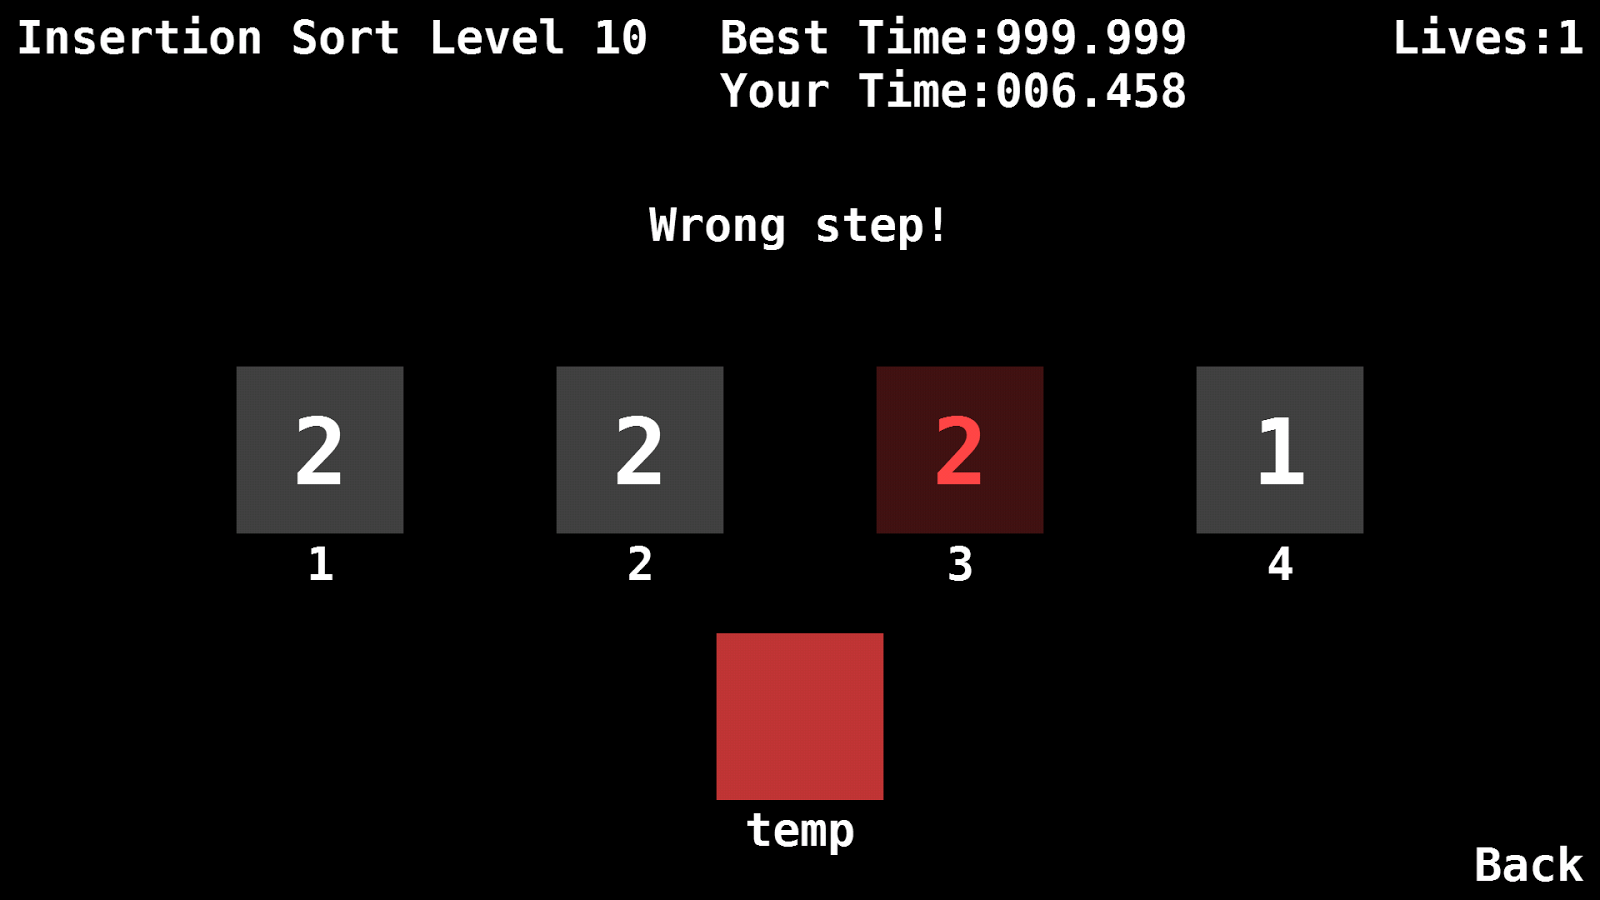
\includegraphics[width=\linewidth]{sort-attack}
  \caption{Sort Attack: Gamification of Sorting Algorithm Learning \cite{yohannis2015sort}.}
  \label{fig:sort-attack}
\end{figure}


We have tested Sort Attack to computer science, informatics, or information technology students with the details of the test method explained in our previous work \cite{yohannis2015sort}. We have performed three instances of the test at three different universities to support the generality of our findings. In brief, the test was a controlled experiment consisting of two sessions and two groups of students. At the first session, a group learned sorting algorithms using textbooks only as the resources of their learning materials and a group that used Sort Attack as their learning tool. After a 15-minute learning, they were asked to solve sorting algorithms problems. After a while, they were requested to change their mode of learning and were given further 15 minutes to study the sorting algorithms before they were again asked to solve other sorting algorithms problems. We report the result of the first test in our previous publication \cite{yohannis2015sort}.

Before ending the test, students were asked to upload their event logs using the upload log feature inside Sort Attack (Table \ref{tab:log} shows a sample format of the event logs). We explained that the logs will be useful for our further research, but they were not obligated. After two months, 60 log files were uploaded. Next, we reviewed the log’s size; we decided to remove two logs from our collection since the size is too small and no significant information was contained in the logs, leaving us with 58 log files to study. The format of the log was explained in our previous work \cite{yohannis2015visualization} with every line record containing information on the state, activity, and time of the event. From the log, we can reconstruct a graph of how a learner plays the artefact and also  identify sixteen attributes that can be associated to measure the behaviours and performance of a learner’s learning processes. 

\begin{table}[]
  \centering
  \caption{A sample format of event log generated in Sort Attack \cite{yohannis2015visualization}.}
  \label{tab:log}
  \begin{tabular}{p{.02\linewidth} p{.2\linewidth} p{.62\linewidth}}
    \hline
    \textbf{Id} & \textbf{Timestamp} & \textbf{Label}                                                                                                         \\ \hline
    001         & 18032015102433     & Insertion Sort Level 13: Level Started                                                                                 \\
    001         & 18032015102436     & Insertion   Sort Level 13: Fail - Dropped box 2 to box holder -1, dropped box 1 to box   holder -1 expected, Lives = 2 \\
    001         & 18032015102438     & Insertion   Sort Level 13: Success - 1 to -1                                                                           \\
    001         & 18032015102439     & Insertion Sort Level 13: Fail - Dropped box 1 to box holder 2, dropped box 2 to box holder 2 expected, Lives = 1       \\ \hline
  \end{tabular}
\end{table}

We assume a log file is a representation of a learner who played with the artefact since the log file recorded the person’s activities with the artefact. A change in one of the attributes of the person’s interaction with the artefact might have certain relationships with the changes in other attributes. Therefore, we use correlation approach to identify the relationships between the attributes.  We use the 58 learners as the number of measurements required for the correlation calculation. We proceeded to do a normality test using the Shapiro-Wilk test \cite{shapiro1965variance} on every attribute and identified that not all attributes have a normal distribution. Consequently, we used Kendall’s Tau \cite{kendall1938correlation} to calculate the correlation between the attributes.


\section{Results and Discussions}
\label{sec:results_and_discussions}

\subsection{The Attributes of Learners’ Learning Behaviours and Their Grouping}
\label{sec:attributes}

Based on the game logs collected, we have successfully identified sixteen attributes that we classified into three groups: After-Failure Strategies, Learning Efforts, and Learning Outputs. The attributes can be used to describe learners’ learning behaviours and to measure their learning outputs during their interactions with the artefact. 
After-Failure Strategies are the strategies used by learners to overcome their difficulties or failures in completing certain levels. We assume that it is important to understand which strategy is most effective to determine the success of learners to perform well in learning. Therefore, we have identified six after-failure strategies as follows: Theoretical Strategy (THS): Revisit the Introduction (Level 1) after failure, striving to understand the intended algorithm through theoretical explanation. Demo Strategy (DES): Return to Tutorial (Level 2) after failure, endeavouring to understand the intended algorithm through watching demos. Replay Strategy (RPS): Replay the level after failure, striving to complete the intended level through replay. Step-back Strategy (SBS): Return to the previous level after failure, striving to complete a difficult level through learning from the previous level. Cross-Algorithm Resolution (COA): ``Give up!'' Leave the difficult level without completing it and move to another different type of algorithm. Leaving-Off Resolution (LOA): Another type of “Give up!” in which learners decided to move on to a higher level but still on the same type of sorting algorithm without completing the troublesome level, which differentiates LOA from COA.


Learning Efforts are the efforts exerted by learners to learn algorithms and accomplish levels. These attributes indicate whether the learners used much or less time and tried to complete the levels. We have identified four attributes as follows. Theoretical Effort (THE): The number of how many times learners start the Introduction (Level 1) to learn algorithms through theoretical explanation. Demonstrative Effort (DEE): The number of how many times learners start the Tutorial (Level 2) to learn algorithms through watching demos. Playtime (PLT): The duration (time) the learners spent to accomplish levels. Number of Attempts (NAT): The number of how many times learners start playing any levels.

Learning Outputs are the attributes that we perceive as the outputs resulting from the learner’s interaction with the game, which can be used to measure the achievement of their learning processes. The followings are the attributes. Number of Game-Overs (NGO), the number of how many times learners experienced Game Over. Number of Errors (NER): The number of how many times learners experienced failures performing the wrong steps. Number of Completions (NCO): The number of how many times learners completed a level. Number of Levels (NOL): The number of how many different levels completed. There are maximum 96 levels available to complete for all the three sorting algorithms, 32 levels each. Error Rate (ERR): The ratio between the number of how many times learners did wrong steps and the number of how many times learners start playing any levels (ERR = NER / NAT).  Success Rate (SUR): The ratio between the number of how many times a learner completes any level and the number of how many times the learner starts playing any level (SUR = NCO / NAT).


\subsection{Findings and Discussions}
\label{sec:findings_and_discussions}

Based on Kendall’s Tau Correlations between the attributes of learners’ learning behaviours in Table \ref{tab:result}, we found some interesting findings that enlighten us on how learners learn algorithms through playing games. We discuss the results in the following paragraphs.

% Please add the following required packages to your document preamble:
% \usepackage{graphicx}
% \usepackage[table,xcdraw]{xcolor}
% If you use beamer only pass "xcolor=table" option, i.e. \documentclass[xcolor=table]{beamer}
% Please add the following required packages to your document preamble:
% \usepackage{graphicx}
% \usepackage[table,xcdraw]{xcolor}
% If you use beamer only pass "xcolor=table" option, i.e. \documentclass[xcolor=table]{beamer}
\begin{table*}[]
  \centering
  \caption{Kendal’s Tau correlations between the attributes of learners’ learning behaviours.}
  \label{tab:result}
  \resizebox{\textwidth}{!}{%
    \begin{tabular}{|c|rrrrrr|rrrr|rrrrrr|}
      \hline
      & \multicolumn{6}{c|}{\textbf{After-Failure Strategies}} & \multicolumn{4}{c|}{\textbf{Learning Efforts}} & \multicolumn{6}{c|}{\textbf{Learning Outputs}} \\ \cline{2-17} 
      & \multicolumn{1}{c}{\textbf{THS}} & \multicolumn{1}{c}{\textbf{DES}} & \multicolumn{1}{c}{\textbf{RPS}} & \multicolumn{1}{c}{\textbf{SBS}} & \multicolumn{1}{c}{\textbf{LOA}} & \multicolumn{1}{c|}{\textbf{COA}} & \multicolumn{1}{c}{\textbf{THE}} & \multicolumn{1}{c}{\textbf{DEE}} & \multicolumn{1}{c}{\textbf{PLT}} & \multicolumn{1}{c|}{\textbf{NAT}} & \multicolumn{1}{c}{\textbf{NGO}} & \multicolumn{1}{c}{\textbf{NER}} & \multicolumn{1}{c}{\textbf{NCO}} & \multicolumn{1}{c}{\textbf{NOL}} & \multicolumn{1}{c}{\textbf{ERR}} & \multicolumn{1}{c|}{\textbf{SUR}} \\ \hline
      \textbf{THS} & 1 & 0.131 & .477** & 0.098 & 0.22 & .310** & .488** & .252* & .281** & .481** & .466** & .538** & .320** & .319** & .298** & -.234* \\
      \textbf{sig.} &  & 0.255 & 0 & 0.345 & 0.051 & 0.003 & 0 & 0.013 & 0.003 & 0 & 0 & 0 & 0.001 & 0.001 & 0.002 & 0.014 \\
      \textbf{DES} & 0.131 & 1 & 0.135 & 0.2 & 0.07 & 0.155 & .298** & .359** & 0.189 & .270* & 0.161 & .217* & 0.189 & 0.125 & 0.02 & -0.083 \\
      \textbf{sig.} & 0.255 &  & 0.23 & 0.093 & 0.588 & 0.199 & 0.007 & 0.002 & 0.084 & 0.013 & 0.151 & 0.047 & 0.083 & 0.257 & 0.858 & 0.445 \\
      \textbf{RPS} & .477** & 0.135 & 1 & .255* & .320** & 0.174 & .399** & .210* & .381** & .442** & .513** & .562** & .258** & .220* & .361** & -.332** \\
      \textbf{sig.} & 0 & 0.23 &  & 0.012 & 0.004 & 0.09 & 0 & 0.033 & 0 & 0 & 0 & 0 & 0.006 & 0.018 & 0 & 0 \\
      \textbf{SBS} & 0.098 & 0.2 & .255* & 1 & .269* & .377** & 0.149 & .270** & .282** & .253* & .557** & .504** & .263** & .233* & .378** & 0.02 \\
      \textbf{sig.} & 0.345 & 0.093 & 0.012 &  & 0.021 & 0.001 & 0.137 & 0.01 & 0.004 & 0.01 & 0 & 0 & 0.008 & 0.019 & 0 & 0.839 \\
      \textbf{LOA} & 0.22 & 0.07 & .320** & .269* & 1 & .302* & .258* & 0.175 & 0.047 & .266* & .445** & .392** & 0.13 & 0.094 & .301** & -0.121 \\
      \textbf{sig.} & 0.051 & 0.588 & 0.004 & 0.021 &  & 0.011 & 0.017 & 0.123 & 0.657 & 0.013 & 0 & 0 & 0.225 & 0.38 & 0.005 & 0.257 \\
      \textbf{COA} & .310** & 0.155 & 0.174 & .377** & .302* & 1 & .295** & 0.125 & 0.074 & .220* & .486** & .435** & 0.113 & 0.088 & .390** & -.210* \\
      \textbf{sig.} & 0.003 & 0.199 & 0.09 & 0.001 & 0.011 &  & 0.003 & 0.237 & 0.46 & 0.027 & 0 & 0 & 0.259 & 0.382 & 0 & 0.035 \\ \hline
      \textbf{THE} & .488** & .298** & .399** & 0.149 & .258* & .295** & 1 & .551** & .421** & .638** & .304** & .399** & .459** & .394** & 0.015 & -0.166 \\
      \textbf{sig.} & 0 & 0.007 & 0 & 0.137 & 0.017 & 0.003 &  & 0 & 0 & 0 & 0.001 & 0 & 0 & 0 & 0.866 & 0.07 \\
      \textbf{DEE} & .252* & .359** & .210* & .270** & 0.175 & 0.125 & .551** & 1 & .409** & .600** & 0.147 & .280** & .583** & .524** & -0.124 & 0.073 \\
      \textbf{sig.} & 0.013 & 0.002 & 0.033 & 0.01 & 0.123 & 0.237 & 0 &  & 0 & 0 & 0.134 & 0.004 & 0 & 0 & 0.195 & 0.445 \\
      \textbf{PLT} & .281** & 0.189 & .381** & .282** & 0.047 & 0.074 & .421** & .409** & 1 & .595** & .228* & .381** & .584** & .528** & 0.022 & 0.08 \\
      \textbf{sig.} & 0.003 & 0.084 & 0 & 0.004 & 0.657 & 0.46 & 0 & 0 &  & 0 & 0.014 & 0 & 0 & 0 & 0.804 & 0.376 \\
      \textbf{NAT} & .481** & .270* & .442** & .253* & .266* & .220* & .638** & .600** & .595** & 1 & .339** & .511** & .739** & .678** & 0.045 & -0.016 \\
      \textbf{sig.} & 0 & 0.013 & 0 & 0.01 & 0.013 & 0.027 & 0 & 0 & 0 &  & 0 & 0 & 0 & 0 & 0.619 & 0.862 \\ \hline
      \textbf{NGO} & .466** & 0.161 & .513** & .557** & .445** & .486** & .304** & 0.147 & .228* & .339** & 1 & .801** & .202* & .200* & .680** & -.199* \\
      \textbf{sig.} & 0 & 0.151 & 0 & 0 & 0 & 0 & 0.001 & 0.134 & 0.014 & 0 &  & 0 & 0.03 & 0.032 & 0 & 0.032 \\
      \textbf{NER} & \cellcolor[HTML]{EFEFEF}.538** & .217* & \cellcolor[HTML]{EFEFEF}.562** & \cellcolor[HTML]{EFEFEF}.504** & \cellcolor[HTML]{EFEFEF}.392** & \cellcolor[HTML]{EFEFEF}.435** & \cellcolor[HTML]{EFEFEF}.399** & \cellcolor[HTML]{EFEFEF}.280** & \cellcolor[HTML]{EFEFEF}.381** & \cellcolor[HTML]{EFEFEF}.511** & \cellcolor[HTML]{EFEFEF}.801** & 1 & \cellcolor[HTML]{EFEFEF}.369** & \cellcolor[HTML]{EFEFEF}.358** & \cellcolor[HTML]{EFEFEF}.536** & -0.141 \\
      \textbf{sig.} & \cellcolor[HTML]{EFEFEF}0 & 0.047 & \cellcolor[HTML]{EFEFEF}0 & \cellcolor[HTML]{EFEFEF}0 & \cellcolor[HTML]{EFEFEF}0 & \cellcolor[HTML]{EFEFEF}0 & \cellcolor[HTML]{EFEFEF}0 & \cellcolor[HTML]{EFEFEF}0.004 & \cellcolor[HTML]{EFEFEF}0 & \cellcolor[HTML]{EFEFEF}0 & \cellcolor[HTML]{EFEFEF}0 &  & \cellcolor[HTML]{EFEFEF}0 & \cellcolor[HTML]{EFEFEF}0 & \cellcolor[HTML]{EFEFEF}0 & 0.121 \\
      \textbf{NCO} & \cellcolor[HTML]{EFEFEF}.320** & 0.189 & \cellcolor[HTML]{EFEFEF}.258** & \cellcolor[HTML]{EFEFEF}.263** & 0.13 & 0.113 & \cellcolor[HTML]{EFEFEF}.459** & \cellcolor[HTML]{EFEFEF}.583** & \cellcolor[HTML]{EFEFEF}.584** & \cellcolor[HTML]{EFEFEF}.739** & \cellcolor[HTML]{EFEFEF}.202* & \cellcolor[HTML]{EFEFEF}.369** & 1 & \cellcolor[HTML]{EFEFEF}.891** & -0.066 & \cellcolor[HTML]{EFEFEF}.249** \\
      \textbf{sig.} & \cellcolor[HTML]{EFEFEF}0.001 & 0.083 & \cellcolor[HTML]{EFEFEF}0.006 & \cellcolor[HTML]{EFEFEF}0.008 & 0.225 & 0.259 & \cellcolor[HTML]{EFEFEF}0 & \cellcolor[HTML]{EFEFEF}0 & \cellcolor[HTML]{EFEFEF}0 & \cellcolor[HTML]{EFEFEF}0 & \cellcolor[HTML]{EFEFEF}0.03 & \cellcolor[HTML]{EFEFEF}0 &  & \cellcolor[HTML]{EFEFEF}0 & 0.464 & \cellcolor[HTML]{EFEFEF}0.006 \\
      \textbf{NOL} & \cellcolor[HTML]{EFEFEF}.319** & 0.125 & \cellcolor[HTML]{EFEFEF}.220* & \cellcolor[HTML]{EFEFEF}.233* & 0.094 & 0.088 & \cellcolor[HTML]{EFEFEF}.394** & \cellcolor[HTML]{EFEFEF}.524** & \cellcolor[HTML]{EFEFEF}.528** & \cellcolor[HTML]{EFEFEF}.678** & \cellcolor[HTML]{EFEFEF}.200* & \cellcolor[HTML]{EFEFEF}.358** & \cellcolor[HTML]{EFEFEF}.891** & 1 & -0.059 & \cellcolor[HTML]{EFEFEF}.296** \\
      \textbf{sig.} & \cellcolor[HTML]{EFEFEF}0.001 & 0.257 & \cellcolor[HTML]{EFEFEF}0.018 & \cellcolor[HTML]{EFEFEF}0.019 & 0.38 & 0.382 & \cellcolor[HTML]{EFEFEF}0 & \cellcolor[HTML]{EFEFEF}0 & \cellcolor[HTML]{EFEFEF}0 & \cellcolor[HTML]{EFEFEF}0 & \cellcolor[HTML]{EFEFEF}0.032 & \cellcolor[HTML]{EFEFEF}0 & \cellcolor[HTML]{EFEFEF}0 &  & 0.519 & \cellcolor[HTML]{EFEFEF}0.001 \\
      \textbf{ERR} & \cellcolor[HTML]{EFEFEF}.298** & 0.02 & \cellcolor[HTML]{EFEFEF}.361** & \cellcolor[HTML]{EFEFEF}.378** & \cellcolor[HTML]{EFEFEF}.301** & \cellcolor[HTML]{EFEFEF}.390** & 0.015 & -0.124 & 0.022 & 0.045 & \cellcolor[HTML]{EFEFEF}.680** & \cellcolor[HTML]{EFEFEF}.536** & -0.066 & -0.059 & 1 & \cellcolor[HTML]{EFEFEF}-.262** \\
      \textbf{sig.} & \cellcolor[HTML]{EFEFEF}0.002 & 0.858 & \cellcolor[HTML]{EFEFEF}0 & \cellcolor[HTML]{EFEFEF}0 & \cellcolor[HTML]{EFEFEF}0.005 & \cellcolor[HTML]{EFEFEF}0 & 0.866 & 0.195 & 0.804 & 0.619 & \cellcolor[HTML]{EFEFEF}0 & \cellcolor[HTML]{EFEFEF}0 & 0.464 & 0.519 &  & \cellcolor[HTML]{EFEFEF}0.004 \\
      \textbf{SUR} & \cellcolor[HTML]{EFEFEF}-.234* & -0.083 & \cellcolor[HTML]{EFEFEF}-.332** & 0.02 & -0.121 & \cellcolor[HTML]{EFEFEF}-.210* & -0.166 & 0.073 & 0.08 & -0.016 & \cellcolor[HTML]{EFEFEF}-.199* & \cellcolor[HTML]{EFEFEF}-0.141 & \cellcolor[HTML]{EFEFEF}.249** & \cellcolor[HTML]{EFEFEF}.296** & \cellcolor[HTML]{EFEFEF}-.262** & 1 \\
      \textbf{sig.} & \cellcolor[HTML]{EFEFEF}0.014 & 0.445 & \cellcolor[HTML]{EFEFEF}0 & 0.839 & 0.257 & \cellcolor[HTML]{EFEFEF}0.035 & 0.07 & 0.445 & 0.376 & 0.862 & \cellcolor[HTML]{EFEFEF}0.032 & \cellcolor[HTML]{EFEFEF}0.121 & \cellcolor[HTML]{EFEFEF}0.006 & \cellcolor[HTML]{EFEFEF}0.001 & \cellcolor[HTML]{EFEFEF}0.004 &  \\ \hline
    \end{tabular}%
  }
\flushright 
\scriptsize
**significant at the 0.01 level (2-tailed), *significant at the 0.05 level (2-tailed)
\end{table*}

Success Rate (SUR) has significant positive weak correlations with the Number of Completions (NCO) and the Number of Levels (NOL). The interpretation of this finding is that more successes in completing levels or more levels completed indicate a slight increase in success rate. However, playing many times (NAT) or spending more time (PLT) with the artefact does not necessarily predict an increase in Success Rate (SUR). The reason is that learners also experience failures, not only successes, during the learners’ playtime (PLT) and attempts (NAT). Using the playtime and efforts to learn the theories (THE) and viewing the demos (DEE) does not necessarily indicate an increase in Success Rate (SUR) since the playtime (PLT) and attempts (NAT) are used to learn and are not used to complete any levels successfully. Error Rate (ERR) has a significant negative weak correlation with Success Rate (SUR). Thus, an increase in Error Rate (ERR) will indicate a decrease in Success Rate (SUR). The After-Failure Resolutions—the Theoretical Strategy (THS), Replay Strategy (RPS), and Cross-Algorithm Resolution (CAR)—strengthen these reasons. They show significant negative weak to moderate correlations towards the Success Rate, but indicate significant positive moderate relationships towards the Error Rate in opposition.

Number of Levels (NOL) has a significant positive very strong correlation with the Number of Completions (NCO). Therefore, a learner who completed all or most of the levels tends to have a high Number of Completions (NCO) and \textit{vice versa}. Every attribute of Learning Efforts has a significant positive relationship to Number of Levels (NOL): a moderate degree of Theoretical Effort (THE) and a strong degree of Number of Attempts (NAT), with the latter has the strongest relationship with Number of Levels (NOL). These relationships mean that every learning effort exerted will give a significant positive contribution for a learner to complete most or all of the levels. However, the Number of Attempts (NAT) is the strongest predictor to successfully complete the game. 
The best strategy to use when a learner experiences failures in completing certain levels and wants to increase the number of completed levels is through Theoretical Strategy (THS)—return to the theoretical explanation provided in Level 1. This strategy has the most significant positive near moderate correlation to Number of Levels (NOL) compared to other After-Failure Strategies. Other strategies, Replay Strategy (RPS) and Step-back Strategy (SBS) can also be used since they have significant positive correlations with Number of Levels (NOL), despite their strengths are weaker than Theoretical Strategy (THS).

Similar to Number of Levels (NOL), attributes that correlate significantly with Number of Levels also correlate significantly with Number of Completions (NCO), except that their correlations’ strengths to the Number of Completions are slightly stronger than their correlations to Number of Levels (excluding Success Rate (SUR) attribute that is slightly weaker). Therefore, Theoretical Effort (THE), Demonstrative Effort (DEE), Playtime (PLT), Number of Attempts (NAT), Theoretical Strategy (THS), Replay Strategy (RPS), and Step-back Strategy (SBS) contribute stronger, positively and significantly, to the prediction of Number of Completions (NCO) rather than to the prediction of Number of Levels (NOL).

We also found that Error Rate (ERR) does not correlate significantly with Number of Completions (NCO) and Number of Levels (NOL). It means that having a change in Number of Completions (NCO) or Number of Levels (NOL) does not predict a change in the Error Rate. The explanation here is that there are two possibilities when a learner completes a level; whether the learner can finish the level by making one or more mistakes or without making any mistake at all. The likelihood of these possibilities to occur are of equal chances. When the player moves to a higher level, the person is introduced to new difficulties that increases the possibility of making many mistakes, but the person will increase the possibility of completing the level after playing several times and thus reducing the mistakes made. This explanation is also supported by the insignificant close-to-zero correlations that Error Rate (ERR) has with Number of Completions (NOC) and Number of Levels (NOL). In addition, Error Rate (ERR) can be significantly predicted by Number of Game-Overs (NGO) (0.680**) and Number or Errors (NER) (0.536**). An increase in one of both Number of Game-Overs (NGO) and Number or Errors (NER) positively and strongly predicts an increase in the Error Rate (ERR).  The summary of our findings is shown in  Fig. \ref{fig:conclusion}. The figure shows the simplified relationships between the variables (it only displays relevant variables).


\section{Conclusions}
\label{sec:conclusions}

Based on the findings in the context of our research, we conclude that to have a higher rate of completing a level, we can increase the number of the completed levels and the frequency of the levels completed. To increase them, learners need to dedicate their efforts to understanding the algorithms theoretically, pay attention to the demos or illustrations, spend more time playing, and exert more attempts to complete the levels, with the latter having the strongest magnitude in predicting the frequency of level completions and completing all the levels. 

\begin{figure}
  \centering
  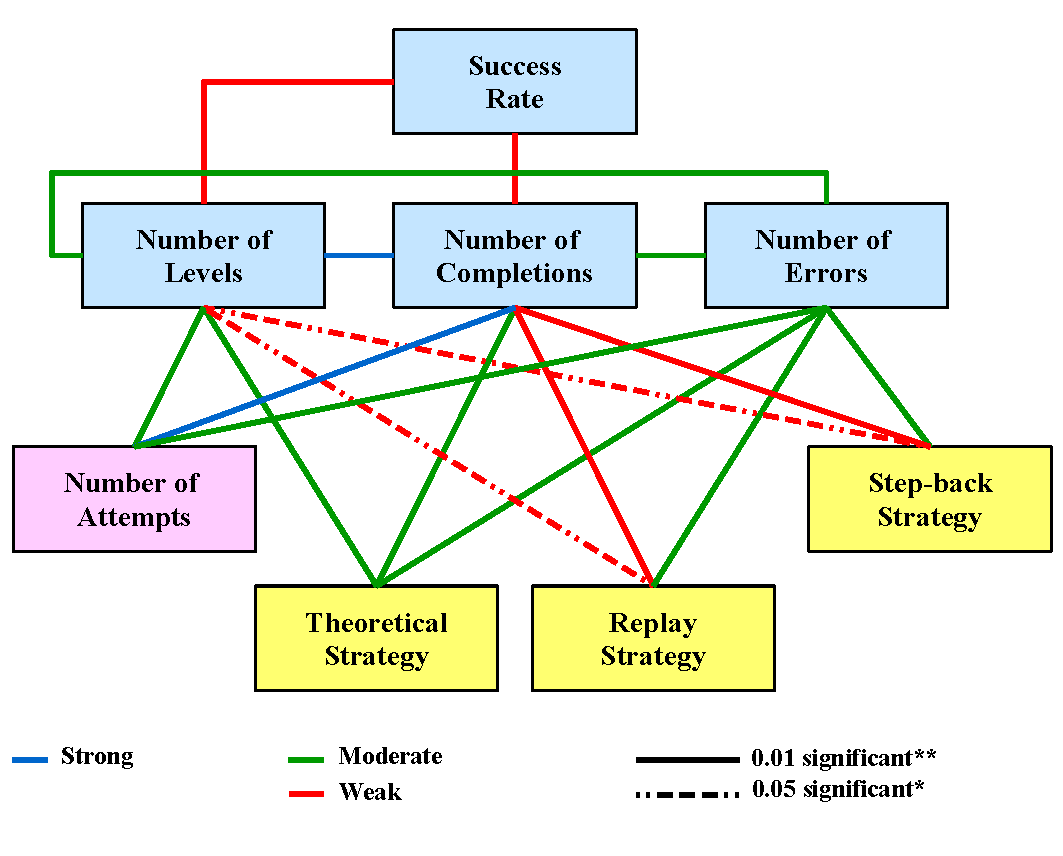
\includegraphics[width=\linewidth]{conclusion}
  \caption{Summary of the correlations between the variables of learning behaviours and learning outcomes after learning using Sort Attack.}
  \label{fig:conclusion}
\end{figure}

When learners make mistakes or experience failures, the best way to overcome the problems is by returning to review the theoretical explanation. It is a type of didactic learning \cite{Austin2013} in which one tries to learn certain topics through the explanation that have been provided by others. This method, in certain situations, is efficient since we do not have to build the knowledge from scratch through iterative experimentation as implied by pure constructivism \cite{McComas2014} and pure experiential learning \cite{kolb2014experiential}. Other two constructivism-like approaches, repetitively retry a level and learning from previous levels exerting trial-and-error approach \cite{Fitzgerald2009} or associative learning \cite{Jozefowiez2012} can also be applied. It is imperative to note that their effects are not as strong as the effect of learning from the theoretical explanation.

Additionally, experiencing failures does not always mean a bad thing since making mistakes is always a part of a learning process. The number of errors we made correlates positively, moderately, and significantly with the number of efforts we put forth when we learn something new. In the end, constant and repetitive efforts to learn something new will lead us to success.

Therefore, for design implications, we need to design games that allow learners to make mistakes, retry, and repetitively learn from their previous failures until they are proficient enough to generate successes in their learning. The design also focuses on the need to allow the learners to learn from the previous levels. Learners may experience this levels to be easier than the difficult ones. This helps in the way we build our capability by learning from the slightly easier challenge to tackle a more challenging one. Most games nowadays already accommodated these kinds of design. They do allow many retries, so players can learn from failures. However, the findings about the after-failure strategies can certainly help in designing stronger Serious Games. For an example, the design needs to provide some theoretical explanation in which learners can revisit after experiencing failures. In this way, they can develop their understanding didactically through the explanation already provided by the tutors. 


\section*{Acknowledgment}

We would like to give our thanks to the students of Information Technology, Computer Science, and Informatics Departments of Universitas Tarumanagara, KALBIS Institute, and Universitas Krida Wacana. This research was funded by KALBIS Institute. Sort Attack can be downloaded from \url{https://apkpure.com/sort-attack/com.gamefulgrowth.sortattack.android}.

\bibliographystyle{IEEEtran}
\bibliography{references}


\end{document}
